%% talk_siam_2026.tex — SIAM conference, 25-minute talk
%% "Covariant Formulation of Shock Waves Propagation
%%  for Traffic Flow on Curved Roads"
%%
\documentclass[aspectratio=169,11pt]{beamer}

\usetheme{default}
\usecolortheme{rose}
\usefonttheme{professionalfonts}
\useinnertheme{rectangles}
\setbeamertemplate{navigation symbols}{}
\setbeamertemplate{footline}[frame number]

\usepackage{amsmath,amssymb,bm}
\usepackage{graphicx}
\usepackage{booktabs}
\usepackage{xcolor}
\usepackage{tikz}
\usetikzlibrary{arrows.meta,decorations.pathmorphing}

\definecolor{C1}{RGB}{0,60,120}
\definecolor{C2}{RGB}{180,30,30}
\definecolor{C3}{RGB}{0,110,55}
\definecolor{C4}{RGB}{170,120,0}
\definecolor{Cg}{RGB}{90,90,90}

\setbeamercolor{frametitle}{bg=C1,fg=white}
\setbeamercolor{block title}{bg=C1!80,fg=white}
\setbeamercolor{block body}{bg=C1!8}
\setbeamercolor{alerted text}{fg=C2}
\setbeamercolor{example text}{fg=C3}
\setbeamerfont{frametitle}{size=\large,series=\bfseries}

\newcommand{\vp}{\varphi}
\newcommand{\mcite}[1]{{\scriptsize\color{Cg}[#1]}}

\title[Shock Waves on Curved Roads]{%
  Covariant Formulation of Shock Waves Propagation\\
  for Traffic Flow on Curved Roads}
\author{H\'ector Medel Cobaxin}
\institute{Escuela de Ingenier\'ia y Ciencias, Tecnol\'ogico de Monterrey, Mexico}
\date{SIAM Conference, May 2026}

% ========================================================================
\begin{document}

% --- SLIDE 1: Title ---
\begin{frame}
  \begin{tikzpicture}[remember picture,overlay]
    \node[anchor=north west,inner sep=8pt] at (current page.north west) {%
      \includegraphics[height=1.1cm]{tecnologico-de-monterrey-blue-eps-converted-to.pdf}%
    };
  \end{tikzpicture}
  \titlepage
\end{frame}

% ====================================================================
\section{Motivation}
% ====================================================================

% --- SLIDE 2: The problem ---
\begin{frame}{Traffic jams on curved roads}
\begin{columns}[T]
  \column{0.50\textwidth}
  \vspace{10pt}
  {\large Traffic waves propagate on \alert{real road geometry}\\
  --- curves, hills, ramps ---\\
  but models assume \textbf{flat space}.}

  \bigskip
  \begin{itemize}
    \setlength\itemsep{8pt}
    \item Empirical evidence: slower flow at sharp turns,
          jam accumulation on inclines
    \item Highway Capacity Manual adjusts capacity
          for curvature --- but \emph{ad hoc}
    \item No first-principles coupling of geometry to
          shock dynamics
  \end{itemize}

  \column{0.46\textwidth}
  \vspace{4pt}
  \begin{center}
  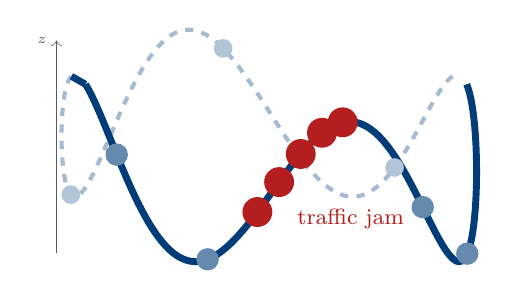
\begin{tikzpicture}[scale=1.35]
    \draw[C1!35,line width=1.5pt,dashed,samples=120,domain=5:175,smooth]
      plot ({1.8*cos(\x) - 0.42*1.8*sin(\x)},
           {0.24*1.8*sin(\x) + 0.72*cos(4*\x)});
    \draw[C1,line width=2.5pt,samples=120,domain=185:355,smooth]
      plot ({1.8*cos(\x) - 0.42*1.8*sin(\x)},
           {0.24*1.8*sin(\x) + 0.72*cos(4*\x)});
    \draw[C1,line width=2.5pt] ({1.8*cos(175)-0.42*1.8*sin(175)},
           {0.24*1.8*sin(175)+0.72*cos(700)})
      -- ({1.8*cos(185)-0.42*1.8*sin(185)},
          {0.24*1.8*sin(185)+0.72*cos(740)});
    \foreach \a in {200,230,295,320}{
      \fill[C1!60] ({1.8*cos(\a)-0.42*1.8*sin(\a)},
                   {0.24*1.8*sin(\a)+0.72*cos(4*\a)}) circle (3pt);
    }
    \foreach \a in {244,250,256,262,268}{
      \fill[C2] ({1.8*cos(\a)-0.42*1.8*sin(\a)},
                 {0.24*1.8*sin(\a)+0.72*cos(4*\a)}) circle (4pt);
    }
    \foreach \a in {30,80,140}{
      \fill[C1!30] ({1.8*cos(\a)-0.42*1.8*sin(\a)},
                   {0.24*1.8*sin(\a)+0.72*cos(4*\a)}) circle (2.5pt);
    }
    \node[C2,font=\footnotesize,anchor=west] at
      ({1.8*cos(250)-0.42*1.8*sin(250)+0.08},
       {0.24*1.8*sin(250)+0.72*cos(1000)-0.35})
      {traffic jam};
    \draw[Cg,very thin,->] (-2.0,-0.95) -- (-2.0,1.05)
      node[left,font=\tiny] {$z$};
  \end{tikzpicture}
  \end{center}
  {\footnotesize 3D road with spatially varying geometry.
   Vehicles cluster where curvature is high.}
\end{columns}
\end{frame}

% --- SLIDE 3: Sugiyama ---
\begin{frame}{Phantom jams: no bottleneck needed}
\begin{columns}[T]
  \column{0.52\textwidth}
  \medskip
  Sugiyama \emph{et al.} (2008) \mcite{1}:\\[6pt]
  22 cars on a circular track.
  Uniform initial speed.
  \textbf{No traffic lights. No accidents.}\\[8pt]

  Within minutes: a \alert{spontaneous traffic jam}
  propagating \emph{backward} against the flow.

  \medskip
  Even on a \textbf{flat circle} the system is
  unstable to density waves.

  \bigskip
  \textbf{Question:} What happens on a road with
  \alert{spatially varying geometry}?

  \column{0.44\textwidth}
  \vspace{6pt}
  \begin{center}
  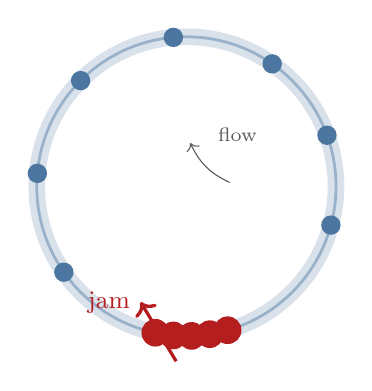
\begin{tikzpicture}[scale=1.0]
    \draw[line width=6pt,C1!15] (0,0) circle (1.9);
    \draw[line width=1pt,C1!40] (0,0) circle (1.9);
    \foreach \a in {20,55,95,135,175,215,345}{
      \fill[C1!70] ({1.9*cos(\a)},{1.9*sin(\a)}) circle (3.5pt);
    }
    \foreach \a in {258,265,272,279,286}{
      \fill[C2] ({1.9*cos(\a)},{1.9*sin(\a)}) circle (5pt);
    }
    \draw[->,C2,very thick]
      ({1.9*cos(260)+0.2},{1.9*sin(260)-0.35})
      -- ({1.9*cos(260)-0.25},{1.9*sin(260)+0.4})
      node[left,font=\small,C2] {jam};
    \draw[->,Cg,thin,bend left=20]
      (0.55,0.05) to (0.05,0.55);
    \node[Cg,font=\scriptsize] at (0.65,0.65) {flow};
  \end{tikzpicture}
  \end{center}
\end{columns}
\end{frame}

% --- SLIDE 4: Prior work and gap ---
\begin{frame}{Prior work and the gap we address}
\begin{columns}[T]
  \column{0.52\textwidth}
  \medskip
  \textbf{What exists:}
  \begin{itemize}
    \setlength\itemsep{4pt}
    \item Conservation laws on Riemannian manifolds:
          well-posedness, FV schemes
          \mcite{2,3}
    \item Traffic on curved roads: lattice and
          macro models with curvature/slope effects
          \mcite{4,5,6}
    \item KdV--Burgers on curved manifolds:
          Laplace--Beltrami dissipation, shock profiles
          \mcite{7}
    \item Embedding methods for conservation
          laws on manifolds in $\mathbb{R}^3$ \mcite{8}
  \end{itemize}

  \column{0.44\textwidth}
  \medskip
  \textbf{What is missing:}

  \begin{alertblock}{The gap}
    No published model combines:
    \begin{enumerate}
      \setlength\itemsep{3pt}
      \item A macroscopic traffic model (LWR)
      \item on a spatial curve $\gamma(s) \in \mathbb{R}^3$
      \item with \alert{explicit} $\kappa(s), \tau(s)$
            in the fundamental diagram
      \item and derives how geometry modifies
            the \textbf{shock velocity}
    \end{enumerate}
  \end{alertblock}

  \smallskip
  {\footnotesize This is what we do.}
\end{columns}
\end{frame}

% ====================================================================
\section{Formulation}
% ====================================================================

% --- SLIDE 5: Curves in R3 ---
\begin{frame}{Spatial curves in $\mathbb{R}^3$: the Frenet--Serret frame}
\begin{columns}[T]
  \column{0.54\textwidth}
  \medskip
  A road is a smooth closed curve $\gamma(s) \in \mathbb{R}^3$
  parametrised by arc length $s$.

  \medskip
  The \textbf{Frenet--Serret apparatus}:
  \begin{align*}
    \mathbf{T}'(s) &= \kappa(s)\,\mathbf{N}(s) \\
    \mathbf{N}'(s) &= -\kappa(s)\,\mathbf{T}(s) + \tau(s)\,\mathbf{B}(s)
  \end{align*}

  \begin{itemize}
    \item $\kappa(s)$: \alert{curvature} (how sharply the road turns)
    \item $\tau(s)$: \alert{torsion} (how the road twists out of plane)
  \end{itemize}

  \medskip
  These are the \textbf{intrinsic geometric data} that
  should couple to flow dynamics.

  \column{0.42\textwidth}
  \vspace{4pt}
  \includegraphics[width=\linewidth]{figures_siam/multi_3d_curves.png}
  \vspace{4pt}
  {\footnotesize Four test geometries: straight line
  ($\kappa=0,\tau=0$), circle ($\kappa=$const, $\tau=0$),
  helix ($\kappa,\tau=$const), modulated 3D curve
  ($\kappa$ varies $\sim 800\times$).}
\end{columns}
\end{frame}

% --- SLIDE 6: Covariant conservation law ---
\begin{frame}{Covariant scalar conservation law}
\begin{columns}[T]
  \column{0.56\textwidth}
  \medskip
  The Lighthill--Whitham--Richards (LWR) equation on a
  \textbf{curved road}:

  \begin{block}{Covariant LWR equation}
    \vspace{4pt}
    \[
      \partial_t \rho + \partial_s\bigl[\rho\,v(\rho;\kappa,\tau)\bigr] = 0
    \]
    \vspace{2pt}
  \end{block}

  \medskip
  The flux depends on geometry via the
  \textbf{fundamental diagram}:
  \[
    v(\rho;\kappa,\tau) = v_{\max}\,
    g(\kappa,\tau)\left(1 - \frac{\rho}{\rho_{\max}}\right)
  \]
  with the \alert{geometric correction}:
  \[
    g(\kappa,\tau) = \exp\!\bigl(-\beta_\kappa|\kappa|
    - \beta_\tau|\tau|\bigr)
  \]

  \column{0.40\textwidth}
  \vspace{4pt}
  \includegraphics[width=\linewidth,height=0.6\textheight,keepaspectratio]%
    {figures_siam/siam_fundamental_4geom.png}
  \vspace{2pt}
  {\footnotesize Fundamental diagrams (LWR) for the four
  geometries. Curvature reduces max flux by $2.0\%$;
  torsion adds $0.07\%$.}
\end{columns}
\end{frame}

% --- SLIDE 7: Rankine-Hugoniot ---
\begin{frame}{Rankine--Hugoniot conditions on curved geometry}
\begin{columns}[T]
  \column{0.56\textwidth}
  \medskip
  At a shock discontinuity, the jump condition gives
  the \textbf{shock velocity}:

  \begin{block}{Geometric Rankine--Hugoniot}
    \vspace{2pt}
    \[
      V_{\rm shock}(s) = \frac{f(\rho_R;s) - f(\rho_L;s)}{\rho_R - \rho_L}
    \]
    \vspace{1pt}
    where $f(\rho;s) = \rho\,v(\rho;\kappa(s),\tau(s))$
  \end{block}

  \smallskip
  For \textbf{constant geometry} ($\kappa,\tau$ uniform):
  \begin{itemize}
    \item $V_{\rm shock} = v_{\max}\,g\,(1 - \rho_L - \rho_R)$
    \item Exact prediction: no free parameters
  \end{itemize}

  \smallskip
  For \textbf{variable geometry}: $V_{\rm shock}(s)$
  depends on position --- the shock accelerates and
  decelerates as it traverses the road.

  \column{0.40\textwidth}
  \vspace{4pt}
  \includegraphics[width=\linewidth,height=0.6\textheight,keepaspectratio]%
    {figures_siam/analysis_shocks.png}
  \vspace{2pt}
  {\footnotesize Shock analysis across geometries.
  For constant $\kappa,\tau$: theory matches numerics
  to \alert{machine precision}.}
\end{columns}
\end{frame}

% --- SLIDE 8: Effective potential ---
\begin{frame}{The effective potential: why $\partial_s\kappa$ matters}
\vspace{-2pt}
\begin{columns}[T]
  \column{0.56\textwidth}
  \smallskip
  Expanding $\partial_s f$ in the conservation law:
  \[
    \partial_t\rho + \lambda(\rho,s)\,\partial_s\rho
    = \underbrace{-\rho\,v(\rho)\,\partial_s\Phi}_{\text{geometric source}}
  \]

  \begin{block}{Effective potential}
    \vspace{1pt}
    $\Phi(s) = \beta_\kappa|\kappa(s)| + \beta_\tau|\tau(s)|$
    \vspace{1pt}
  \end{block}

  \smallskip
  \textbf{Physical interpretation:}
  \begin{itemize}
    \setlength\itemsep{3pt}
    \item $\partial_s\Phi > 0$ (increasing curvature):
          density \alert{accumulates}
    \item $\partial_s\Phi < 0$ (decreasing curvature):
          density depletes
    \item $\partial_s\Phi = 0$ (constant geometry):
          \textbf{no geometric forcing}
  \end{itemize}

  \column{0.40\textwidth}
  \smallskip
  This explains \textbf{three key observations}:

  \medskip
  \begin{enumerate}
    \setlength\itemsep{5pt}
    \item \textbf{Helix} ($\partial_s\Phi = 0$):
          no jammitons
    \item \textbf{Modulated curve} ($\partial_s\Phi$
          large): density traps in high-$\kappa$ regions
    \item Shocks \alert{refract} across
          $\Phi$-gradients --- analogous to
          Snell's law
  \end{enumerate}
\end{columns}
\end{frame}

% ====================================================================
\section{Numerical method}
% ====================================================================

% --- SLIDE 9: Godunov scheme ---
\begin{frame}{Godunov finite-volume scheme}
\begin{columns}[T]
  \column{0.56\textwidth}
  \medskip
  We solve the covariant LWR equation with a
  \textbf{Godunov scheme} on the arc-length coordinate $s$:

  \medskip
  \begin{enumerate}
    \setlength\itemsep{6pt}
    \item Piecewise-constant reconstruction on each cell
    \item Exact Riemann solver at each interface:\\
          $f^* = f(\rho^*)$ with $\rho^*$ from the
          local Rankine--Hugoniot condition
    \item Conservative update:
          \[
            \rho_j^{n+1} = \rho_j^n
            - \frac{\Delta t}{\Delta s}
            \bigl(f^*_{j+1/2} - f^*_{j-1/2}\bigr)
          \]
  \end{enumerate}

  \smallskip
  \begin{alertblock}{Mass conservation}
    Relative error $< 10^{-15}$ --- machine precision.
  \end{alertblock}

  \column{0.40\textwidth}
  \vspace{6pt}
  \textbf{Implementation:}
  \begin{itemize}
    \setlength\itemsep{4pt}
    \item Julia package, $\sim$2000 lines
    \item $N_s = 500$ spatial cells
    \item CFL: $\Delta t \leq \Delta s / \max|f'|$
    \item Periodic BCs
    \item Riemann solver uses local $\kappa(s_j),\tau(s_j)$
  \end{itemize}

  \smallskip
  {\footnotesize Also implemented: MUSCL reconstruction
  with TVD limiters (minmod, van~Leer, MC)
  for second-order accuracy.}
\end{columns}
\end{frame}

% ====================================================================
\section{Results}
% ====================================================================

% --- SLIDE 10: Kymographs overview ---
\begin{frame}{Kymographs: shock propagation across geometries}
  \vspace{2pt}
  \begin{center}
  \includegraphics[height=0.72\textheight,width=\linewidth,keepaspectratio]%
    {figures_siam/siam_kymographs_4geom.png}
  \end{center}
  \vspace{2pt}
  {\footnotesize Space-time density maps $\rho(s,t)$ for the four
  test geometries.
  Riemann problem: $\rho_L = 0.2 \to \rho_R = 0.6$.
  \alert{Constant geometry}: uniform shock velocity.
  \alert{Variable geometry}: shock speed modulated by local $\kappa(s)$.}
\end{frame}

% --- SLIDE 11: Constant geometry results ---
\begin{frame}{Constant-geometry validation}
\begin{columns}[T]
  \column{0.54\textwidth}
  \medskip
  For the three constant-geometry cases
  ($v_{\max}=30$, $\beta_\kappa=1$, $\beta_\tau=0.5$):

  \medskip
  \renewcommand{\arraystretch}{1.35}
  \small
  \begin{tabular}{lccr}
    \toprule
    Geometry & $\kappa$ & $\tau$ & $V_{\rm shock}$ \\
    \midrule
    Straight & $0$ & $0$ & $6.000$ (ref.) \\
    Circle ($R\!=\!50$) & $0.02$ & $0$ & $5.881$ \\
    Helix  & $0.02$ & $0.002$ & $5.877$ \\
    \bottomrule
  \end{tabular}
  \normalsize

  \bigskip
  \begin{itemize}
    \setlength\itemsep{5pt}
    \item Numerical $V_{\rm shock}$ matches Rankine--Hugoniot
          to \alert{machine precision} ($< 10^{-15}$)
    \item Curvature alone: $\mathbf{2.0\%}$ slowdown
    \item Adding torsion: additional $\mathbf{0.07\%}$
    \item $g = e^{-\beta_\kappa|\kappa|-\beta_\tau|\tau|}$
          is \textbf{exact} for constant geometry
  \end{itemize}

  \column{0.42\textwidth}
  \vspace{4pt}
  \includegraphics[width=\linewidth,height=0.6\textheight,keepaspectratio]%
    {figures_siam/multi_curvature_torsion.png}
  \vspace{2pt}
  {\footnotesize $\kappa(s)$ and $\tau(s)$
  profiles. The modulated curve
  has $\kappa$ varying by $\sim 800\times$.}
\end{columns}
\end{frame}

% --- SLIDE 12: Modulated curve ---
\begin{frame}{Variable geometry: geometric refraction}
\vspace{-4pt}
\begin{columns}[T]
  \column{0.48\textwidth}
  \includegraphics[width=\linewidth,height=0.58\textheight,keepaspectratio]%
    {figures_siam/multi_all_kymographs.png}
  \vspace{1pt}
  {\scriptsize Kymographs: shock front \alert{bends}
  across regions of different $\kappa$.}

  \column{0.48\textwidth}
  \includegraphics[width=\linewidth,height=0.58\textheight,keepaspectratio]%
    {figures_siam/multi_comprehensive_summary.png}
  \vspace{1pt}
  {\scriptsize Density evolution, shock trajectories,
  and velocity modulation on the modulated curve.}
\end{columns}

\vspace{2pt}
{\footnotesize
Modulated circle: $\kappa \in [0.05, 40]$, velocity field $v \in [0, 13.6]$ ---
\textbf{1700\% variation}.
Shocks \textbf{nearly halt} at high $\kappa$ and \textbf{accelerate}
through low-$\kappa$ stretches.
This is the \alert{geometric refraction} predicted by the effective potential $\Phi(s)$.}
\end{frame}

% --- SLIDE 13: Connection to microscopic ---
\begin{frame}{Connection to microscopic dynamics}
\begin{columns}[T]
  \column{0.54\textwidth}
  \medskip
  The covariant LWR sits atop a \textbf{three-scale hierarchy}
  that we have verified independently:

  \begin{center}
  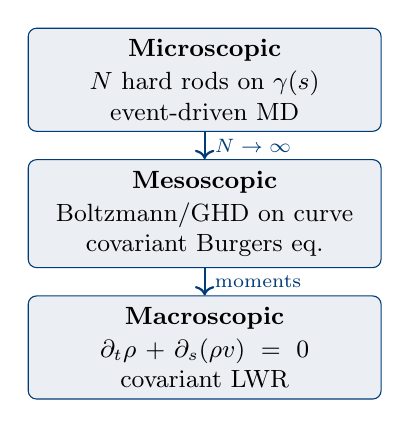
\begin{tikzpicture}[
      box/.style={draw=C1,rounded corners=3pt,
                  fill=C1!8,font=\small,
                  text width=4.2cm,align=center,
                  inner sep=4pt},
      arr/.style={->,C1,thick}]
    \node[box] (micro) at (0,0)
      {\textbf{Microscopic}\\[1pt]$N$ hard rods on $\gamma(s)$\\
       event-driven MD};
    \node[box] (meso) at (0,-1.7)
      {\textbf{Mesoscopic}\\[1pt]Boltzmann/GHD on curve\\
       covariant Burgers eq.};
    \node[box] (macro) at (0,-3.4)
      {\textbf{Macroscopic}\\[1pt]$\partial_t\rho+\partial_s(\rho v)=0$\\
       covariant LWR};
    \draw[arr] (micro) -- node[right,font=\scriptsize]
      {$N\to\infty$} (meso);
    \draw[arr] (meso) -- node[right,font=\scriptsize]
      {moments} (macro);
  \end{tikzpicture}
  \end{center}

  \column{0.42\textwidth}
  \vspace{4pt}
  \includegraphics[width=\linewidth]%
    {../Paper02/figures/fig5_pde_vs_md.pdf}
  \vspace{2pt}
  {\footnotesize \textbf{Lines}: covariant Burgers PDE.
  \textbf{Symbols}: molecular dynamics,
  500 hard rods on an ellipse.
  \alert{24 initial conditions},
  no free parameters.}

  \vspace{2pt}
  {\footnotesize Elastic hard rods
  \alert{do not} form Burgers shocks ---
  shocks require the macroscopic closure.}
\end{columns}
\end{frame}

% --- SLIDE 14: Arc-length universality ---
\begin{frame}{Arc-length universality}
\begin{columns}[T]
  \column{0.54\textwidth}
  \medskip
  \textbf{Key theoretical property:}

  \medskip
  In arc-length coordinates $s$, the covariant equation
  reduces to \textbf{flat-space LWR} with a
  position-dependent fundamental diagram.

  \medskip
  All exact solutions of flat Burgers
  \emph{transplant} to the curved road:
  \begin{itemize}
    \setlength\itemsep{4pt}
    \item N-wave $\to$ metric-distorted N-wave
    \item Sawtooth $\to$ metric-modulated sawtooth
    \item Cole--Hopf viscous profile $\to$ curved Cole--Hopf
  \end{itemize}

  \smallskip
  \begin{alertblock}{Consequence}
    Shock dynamics on \emph{any} geometry =
    flat-space theory + local $g(\kappa,\tau)$.
  \end{alertblock}

  \column{0.42\textwidth}
  \vspace{2pt}
  \includegraphics[width=\linewidth,height=0.55\textheight,keepaspectratio]%
    {../Paper02/figures/fig4_pulse_propagation.pdf}
  \vspace{2pt}
  {\footnotesize N-wave on an ellipse: the two fronts
  travel at different speeds --- the pulse
  \alert{distorts asymmetrically}.}
\end{columns}
\end{frame}

% ====================================================================
\section{Summary}
% ====================================================================

% --- SLIDE 15: Summary ---
\begin{frame}{Summary and outlook}
\vspace{-2pt}
\begin{columns}[T]
  \column{0.54\textwidth}
  \textbf{What we showed:}
  \begin{itemize}
    \setlength\itemsep{3pt}
    \item Covariant LWR on curves in $\mathbb{R}^3$
          with $\kappa(s),\tau(s)$ in the flux
    \item Effective potential $\Phi(s)$ governs
          density redistribution
    \item Godunov: mass error $< 10^{-15}$
    \item Constant geometry: \alert{exact} $V_{\rm shock}$
    \item Variable geometry: \alert{geometric refraction}
  \end{itemize}

  \column{0.42\textwidth}
  \textbf{Future work:}
  \begin{itemize}
    \setlength\itemsep{3pt}
    \item Agent-based IDM validation on curves
    \item GPS data on curved highways
    \item Active matter on manifolds
    \item Higher-order MUSCL/WENO schemes
    \item Networks of curved roads
  \end{itemize}
\end{columns}

\vspace{2pt}
\begin{center}
\renewcommand{\arraystretch}{1.05}
\footnotesize
\begin{tabular}{@{}lccl@{}}
  \toprule
  \textbf{Geometry} & $V_{\rm shock}$ & \textbf{Error vs.\ R--H} & \textbf{Effect} \\
  \midrule
  Straight ($\kappa\!=\!0$) & $6.000$ & $0$ (ref.) & --- \\
  Circle ($\kappa\!=\!$const) & $5.881$ & $< 10^{-15}$ & $-2.0\%$ \\
  Helix ($\kappa,\tau\!=\!$const) & $5.877$ & $< 10^{-15}$ & $-2.07\%$ \\
  Modulated ($\kappa$ variable) & varies & pos.-dependent & geom.\ refraction \\
  \bottomrule
\end{tabular}
\normalsize
\end{center}
\end{frame}

% --- SLIDE 16: Thank you ---
\begin{frame}[plain]
  \begin{center}
  \vspace{1.2cm}
  {\Huge\bfseries\color{C1} Thank you!}\\[18pt]
  {\large H\'ector Medel Cobaxin}\\[4pt]
  {\normalsize\texttt{hjmedel@gmail.com}}\\[4pt]
  {\small Tecnol\'ogico de Monterrey}\\[20pt]
  \rule{0.55\linewidth}{0.4pt}\\[12pt]
  {\small
    Questions?
  }
  \end{center}
\end{frame}

% ========================================================================
\appendix

% --- Backup: References ---
\begin{frame}[noframenumbering]{References}
\footnotesize
\renewcommand{\arraystretch}{1.2}
\begin{tabular}{@{}rl@{}}
\mcite{1} & Sugiyama \emph{et al.}, New J.\ Phys.\ \textbf{10}, 033001 (2008) \\
\mcite{2} & Ben-Artzi \& LeFloch, Ann.\ IHP Anal.\ Non Lin.\ \textbf{24}, 989 (2006) \\
\mcite{3} & LeFloch, Okutmustur \& Neves, Acta Math.\ Sinica \textbf{25}, 1041 (2008) \\
\mcite{4} & Zhou \& Shi, Nonlinear Dyn.\ \textbf{83}, 1217 (2016) \\
\mcite{5} & Xue \emph{et al.}, Nonlinear Dyn.\ \textbf{95}, 3295 (2019) \\
\mcite{6} & Tian \& Kang, Symmetry \textbf{17}, 1299 (2025) \\
\mcite{7} & Palencia, ZAMM \textbf{106}, e70435 (2026) \\
\mcite{8} & Wang \emph{et al.}, J.\ Sci.\ Comput.\ \textbf{93}, 56 (2022) \\
\mcite{9} & El \& Hoefer, SIAM Rev.\ \textbf{59}, 3 (2017) \\
\mcite{10} & Lighthill \& Whitham, Proc.\ R.\ Soc.\ A \textbf{229}, 317 (1955) \\
\end{tabular}
\end{frame}

% --- Backup: Parameters and geometry ---
\begin{frame}[noframenumbering]{Backup: Simulation parameters}
\begin{columns}[T]
  \column{0.54\textwidth}
  \medskip
  The geometric correction to the fundamental diagram
  accounts for the reduced effective speed on curves:

  \medskip
  A vehicle on a curve of curvature $\kappa$ experiences
  centripetal acceleration $a_c = v^2\kappa$.
  Stability requires $a_c \leq \mu g_{\rm grav}$,
  giving the speed reduction:
  \[
    v_{\max}(\kappa) = v_{\max}^{\rm flat}
    \sqrt{\frac{\mu g_{\rm grav}}{\kappa}}
    \quad\text{for large }\kappa
  \]

  The exponential model $g = e^{-\beta_\kappa|\kappa|}$
  interpolates smoothly between flat ($\kappa=0$) and
  highly curved regimes.

  \column{0.42\textwidth}
  \medskip
  \textbf{Parameters used:}
  \begin{itemize}
    \setlength\itemsep{4pt}
    \item $v_{\max} = 30.0$
    \item $\rho_{\max} = 1.0$
    \item $\beta_\kappa = 1.0$ (curvature sensitivity)
    \item $\beta_\tau = 0.5$ (torsion sensitivity)
    \item $\alpha = 1$ (Greenshields)
    \item Riemann: $\rho_L = 0.2,\; \rho_R = 0.6$
  \end{itemize}

  \medskip
  \textbf{Test geometries:}
  \begin{itemize}
    \setlength\itemsep{4pt}
    \item Circle: $R=50$, $\kappa = 1/R$, $\tau = 0$
    \item Helix: $R=50$, $h=100$
    \item Modulated: $\gamma(\vp) =
          (a\cos\vp, a\sin\vp, a^2\cos 2\vp)$, $a=10$
  \end{itemize}
\end{columns}
\end{frame}

% --- Backup: Covariant Burgers ---
\begin{frame}[noframenumbering]{Backup: Covariant Burgers equation}
\begin{columns}[T]
  \column{0.54\textwidth}
  \medskip
  From the kinetic hierarchy (moment closure),
  the velocity field satisfies the
  \textbf{covariant Burgers equation}:

  \[
    \partial_t u + u\,\partial_\vp u
    + \Gamma(\vp)\,u^2 = 0
  \]

  where $\Gamma = g'/(2g)$ is the Christoffel symbol
  of the metric $g(\vp) = |\gamma'(\vp)|^2$.

  \medskip
  \textbf{Key property:} in arc-length coordinates
  $s$, the physical velocity $v = \sqrt{g}\,u$
  satisfies the flat Burgers equation.

  \medskip
  This establishes \alert{exact equivalence}
  between curved and flat dynamics up to coordinate
  transformation.

  \column{0.42\textwidth}
  \vspace{4pt}
  \includegraphics[width=\linewidth]%
    {../Paper02/figures/fig6_nwave_distortion.pdf}
  \vspace{4pt}
  {\footnotesize N-wave distortion on the ellipse.
  The Christoffel term $\Gamma u^2$ accelerates
  the wave in low-$g$ regions and decelerates it
  in high-$g$ regions.}
\end{columns}
\end{frame}

\end{document}
